\section{Key Concepts and Terminology}

In this chapter, we will get hands-on experience by writing a smart contract in Aiken and the corresponding off-chain code, typically implemented in the frontend using Mesh. Finally, we will submit a transaction and interact with it.

At the end of the chapter, you will also find exercises to test your understanding and skills.

\subsection{Key Concepts}

Here is a list of key concepts and terminology that will help you:

\begin{itemize}
    \item \textbf{Collateral}: A specific UTxO required to interact with smart contracts. It ensures that nodes are compensated in case the contract validation fails.
    \item \textbf{Script Hash}: A unique hash that identifies the smart contract, allowing transactions to reference it securely.
    \item \textbf{Locked UTxO}: A transaction output that holds funds, NFTs, or tokens locked within a contract. These can only be spent if the contract validation logic passes.
    \item \textbf{CIP69 Contract}: A contract where the datum is optional. It behaves like a user, allowing it to receive funds. However, every UTxO associated with this contract must execute the validation logic to be spendable.
    \item \textbf{Multipurpose Script}: A versatile script that can perform multiple functions, such as locking funds, minting NFTs, and more.
\end{itemize}


\section{Writing Your First Smart Contract}

Let's write and execute a smart contract on Cardano in 10 minutes. Yes, you read that right.

You can find code supporting this tutorial on Aiken's main repository.

\subsection{Covered in this tutorial}
\begin{itemize}
    \item Writing a basic Aiken validator;
    \item Writing \& running tests with Aiken;
    \item Troubleshooting smart contracts.
\end{itemize}

When encountering an unfamiliar syntax or concept, do not hesitate to refer to the language-tour for details and extra examples.

\subsection{Pre-requisites}
We'll use Aiken to write the script, so make sure the command-line tool is installed already. Otherwise, refer to the installation instructions.

\subsection{Scaffolding}
First, let's create a new Aiken project:

\begin{verbatim}
aiken new aiken-lang/hello-world
cd hello-world
\end{verbatim}

This command scaffolds an Aiken project. In particular, it creates a \texttt{lib} and \texttt{validators} folder in which you can put Aiken source files.

\begin{verbatim}
./hello-world
│
├── README.md
├── aiken.toml
├── lib
└── validators
\end{verbatim}

\subsection{Using the standard library}
We'll use the standard library for writing our validator. Fortunately, \texttt{aiken new} did automatically add the standard library to our \texttt{aiken.toml} for us. It should look roughly like that:

\begin{verbatim}
aiken.toml
name = "aiken-lang/hello-world"
version = "0.0.0"
license  = "Apache-2.0"
description = "Aiken contracts for project 'aiken-lang/hello-world'"
 
[repository]
user = 'aiken-lang'
project = 'hello-world'
platform = 'github'
 
[[dependencies]]
name = "aiken-lang/stdlib"
version = "v2"
source = "github"
\end{verbatim}

Now, running \texttt{aiken check}, we should see dependencies being downloaded. That shouldn't take long.

\begin{verbatim}
❯ aiken check
    Compiling aiken-lang/hello-world 1.0.0 (examples/hello-world/)
    Resolving aiken-lang/hello-world
      Fetched 1 package in 0.01s from cache
    Compiling aiken-lang/stdlib v2 (/Users/aiken/Documents/aiken-lang/hello-world/build/packages/aiken-lang-stdlib)
      Summary 0 errors, 0 warnings
\end{verbatim}

\subsection{Our First Validator}
Let's write our first validator as \texttt{validators/hello\_world.ak}:

\begin{verbatim}
validators/hello_world.ak
use aiken/collection/list
use aiken/crypto.{VerificationKeyHash}
use cardano/transaction.{OutputReference, Transaction}
 
pub type Datum {
  owner: VerificationKeyHash,
}
 
pub type Redeemer {
  msg: ByteArray,
}
 
validator hello_world {
  spend(
    datum: Option<Datum>,
    redeemer: Redeemer,
    _own_ref: OutputReference,
    self: Transaction,
  ) {
    expect Some(Datum { owner }) = datum
    let must_say_hello = redeemer.msg == "Hello, World!"
    let must_be_signed = list.has(self.extra_signatories, owner)
    must_say_hello && must_be_signed
  }
}
\end{verbatim}

Our first validator is rudimentary, yet there's already a lot to say about it.

It looks for a verification key hash (\texttt{owner}) in the datum and a message (\texttt{msg}) in the redeemer. Remember that, in the eUTxO model, the datum is set when locking funds in the contract and can be seen as configuration. Here, we'll indicate the owner of the contract and require a signature from them to unlock funds—very much like it already works on a typical non-script address.

Moreover, because there's no "Hello, World!" without a proper "Hello, World!", our little contract also demands this very message, as a UTF-8-encoded byte array, to be passed as redeemer (i.e. when spending from the contract).

It's now time to build our first contract!

\begin{verbatim}
aiken build
\end{verbatim}

This command generates a CIP-0057 Plutus blueprint as \texttt{plutus.json} at the root of your project. This blueprint describes your on-chain contract and its binary interface. In particular, it contains the generated on-chain code that will be executed by the ledger and a hash of your validator(s) that can be used to construct addresses.

This format is framework-agnostic and is meant to facilitate interoperability between tools. The blueprint is fully integrated into Aiken, which can automatically generate it based on your type definitions and comments.

\subsection{Let's see the validator in action!}

\begin{itemize}
    \item Interact with a validator on the Preview network;
    \item Using Mesh through Blockfrost;
    \item Getting test funds from the Cardano Faucet;
    \item Using web explorers such as CardanoScan.
\end{itemize}

\subsection{Pre-requisites}
We assume that you have followed the "Hello, World!"'s First steps and thus, have Aiken installed and ready-to-use. We will also use Mesh, so make sure you have your dev environment ready for some JavaScript!.

You can install Mesh and set up the project as follows:

\begin{verbatim}
npm init -y
npm install @meshsdk/core tsx
\end{verbatim}

\subsection{Getting Funds}
For this tutorial, we will use the validator we built in First steps. Yet, before moving on, we'll need some funds, and a public/private key pair to hold them. We can generate a private key and an address using MeshWallet.

\begin{verbatim}
generate-credentials.ts
import { MeshWallet } from '@meshsdk/core';
import fs from 'node:fs';
 
const secret_key = MeshWallet.brew(true) as string;
 
fs.writeFileSync('me.sk', secret_key);
 
const wallet = new MeshWallet({
  networkId: 0,
  key: {
    type: 'root',
    bech32: secret_key,
  },
});
 
fs.writeFileSync('me.addr', wallet.getUnusedAddresses()[0]);
\end{verbatim}

You can run the instructions above via:

\begin{verbatim}
npx tsx generate-credentials.ts
\end{verbatim}

Now, we can head to the Cardano faucet to get some funds on the preview network to our newly created address (inside \texttt{me.addr}).

Make sure to select "Preview Testnet" as the network.

Using CardanoScan, we can watch for the faucet sending some ADA our way. This should be pretty fast (a couple of seconds).

\section{Deploying and Interacting with Smart Contracts}
No need to deploy like in ethereum, as soon as we send a transaction in the contract we are ready to go.

Now that we have some funds, we can lock them in our newly created contract. We'll use Blockfrost Provider to construct and submit our transaction through Blockfrost.

This is only one example of a possible setup using tools we love. For more tools, make sure to check out the Cardano Developer Portal!

\subsection{Setup}
First, we set up Mesh with Blockfrost as a provider. This will allow us to let Mesh handle transaction building for us, which includes managing changes. It also gives us a direct way to submit the transaction later on.

\begin{verbatim}
common.ts
import fs from "node:fs";
import {
  BlockfrostProvider,
  MeshTxBuilder,
  MeshWallet,
  serializePlutusScript,
  UTxO,
} from "@meshsdk/core";
import { applyParamsToScript } from "@meshsdk/core-csl";
 
const blockchainProvider = new BlockfrostProvider(process.env.BLOCKFROST_PROJECT_ID);
 
// wallet for signing transactions
export const wallet = new MeshWallet({
  networkId: 0,
  fetcher: blockchainProvider,
  submitter: blockchainProvider,
  key: {
    type: "root",
    bech32: fs.readFileSync("me.sk").toString(),
  },
});
\end{verbatim}

Note that the highlighted line above looks for an environment variable named \texttt{BLOCKFROST\_PROJECT\_ID} which its value must be set to your Blockfrost project id. You can define a new environment variable in your terminal by running (in the same session you're also executing the script!):

\begin{verbatim}
export BLOCKFROST_PROJECT_ID=preview...
\end{verbatim}

Replace \texttt{preview...} with your actual project id.

\subsection{Locking Funds into the Contract}
Now that we can read our validator, we can make our first transaction to lock funds into the contract. The datum must match the representation expected by the validator (and as specified in the blueprint), so this is a constructor with a single field that is a byte array.

\begin{verbatim}
lock.ts
import { Asset, deserializeAddress, mConStr0 } from "@meshsdk/core";
import { getScript, getTxBuilder, wallet } from "./common";
 
async function main() {
  // these are the assets we want to lock into the contract
  const lockAmount = 10_000_000;
 
  // get a valid address for the contract
  const validatorAddr = deserializeAddress(
    "addr_test1qxygsw9r9rt5q0jx8m6lmcjlsrn2ck7c7tpekl9wzyj8nvc70wwdlcs78s7ntljtm6xqfvwzttttts33dtjpytldc7cs7dpjl7jqxyr9qyz3e"
  );
 
  // lock the funds!
  const { tx, requiredSigners } = await getTxBuilder().build({
    assets: [new Asset("lovelace", lockAmount)],
    recipients: [
      {
        address: validatorAddr,
        datum: { owner: wallet.getUnusedAddresses()[0] },
      },
    ],
  });
  await wallet.signAndSubmit(tx, requiredSigners);
}
 
main();
\end{verbatim}


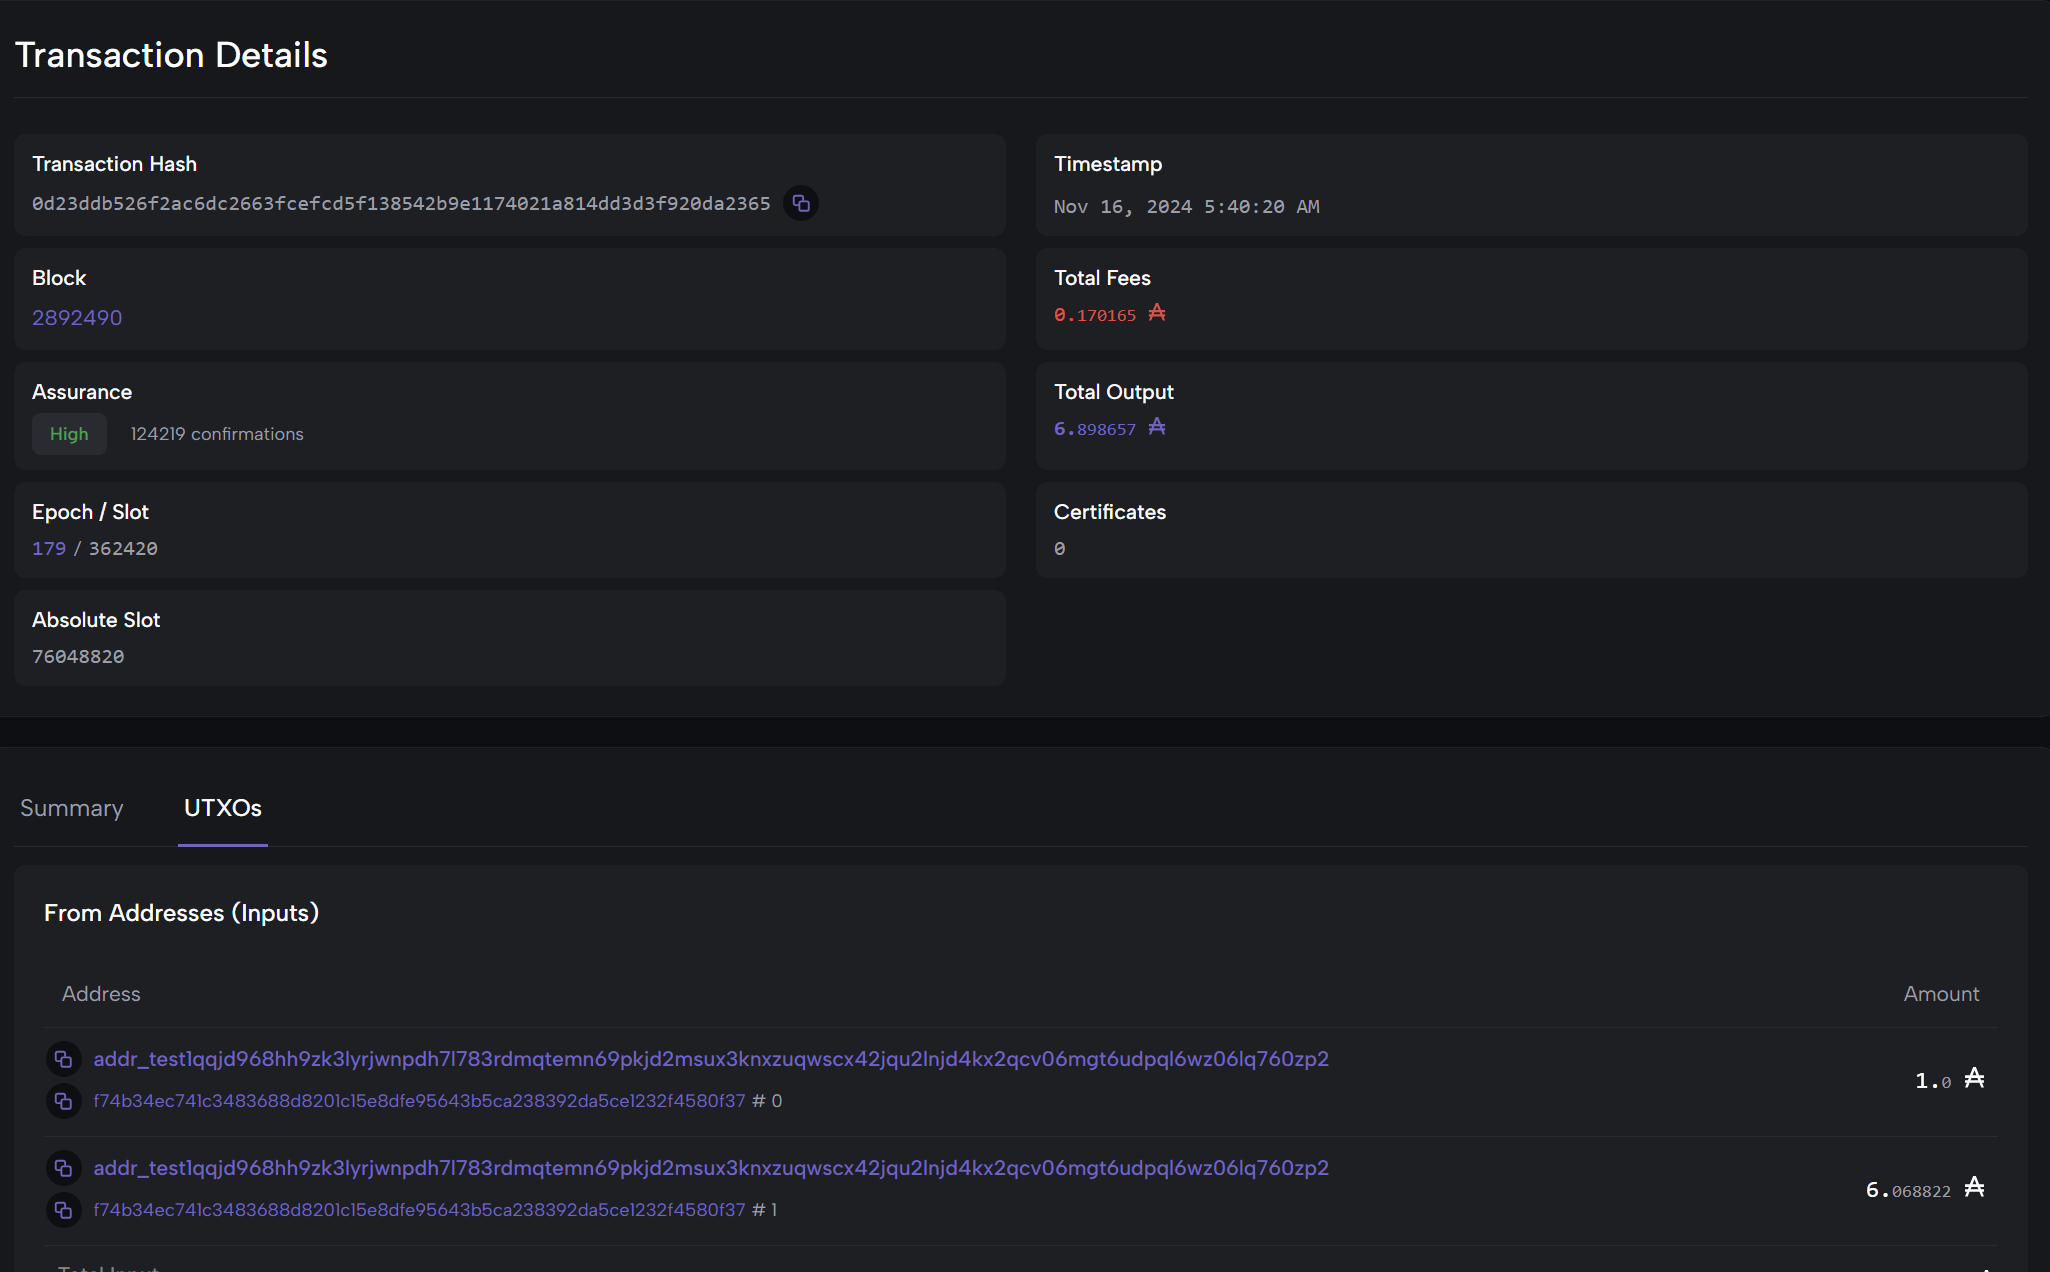
\includegraphics[scale=0.3]{lock.png}


Once again, you may check the transaction on CardanoScan.

\subsection{Spending from the Contract}
With our funds now locked in the contract, we can now spend them. First, we'll need a transaction that spends the funds, passing in the correct redeemer with the value \texttt{Hello, World!}.

\begin{verbatim}
spend.ts
import { getTxBuilder, wallet } from "./common";
 
async function main() {
  const tx = await getTxBuilder().build({
    assets: [{ asset: "lovelace", amount: 10_000_000 }],
    recipients: [
      {
        address: wallet.getUnusedAddresses()[0],
        redeemer: { msg: "Hello, World!" },
      },
    ],
  });
  await wallet.signAndSubmit(tx);
}
 
main();
\end{verbatim}
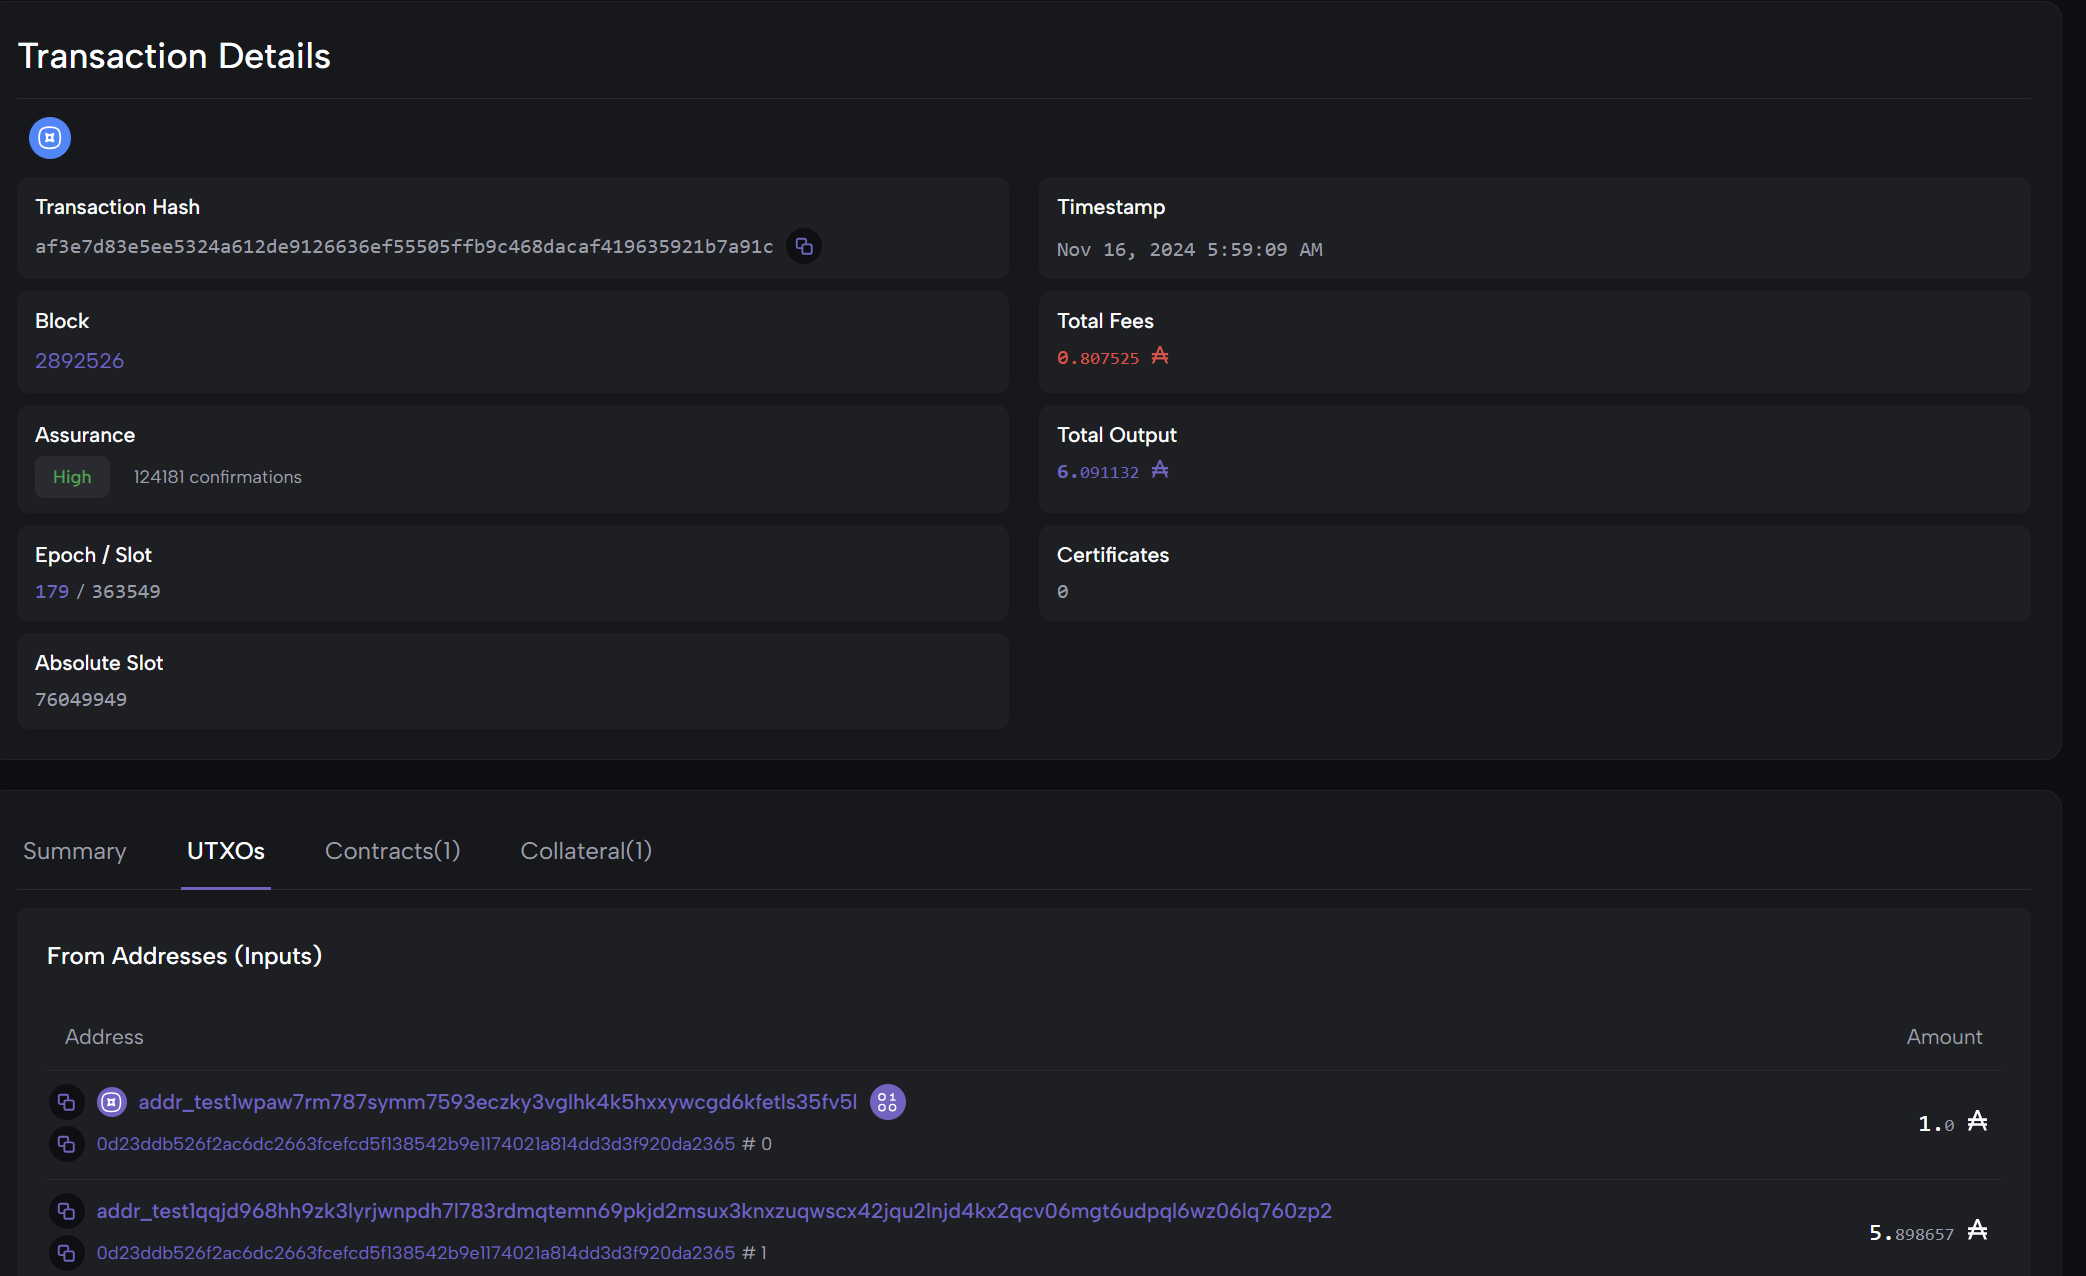
\includegraphics[scale=0.3]{unlock.png}



Once the transaction is complete, go ahead and look for it on CardanoScan again to confirm the transaction has been processed.

You can look for it using the transaction hash: \textit{af3e7d83e5ee5324a612de9126636ef55505ffb9c468dacaf419635921b7a91c}


\section{Best Practices for Secure and Robust Smart Contract}

Auditing should be mandatory before any contract goes live. While open-source code is beneficial for transparency and trust, it is not sufficient on its own. Audits help identify potential vulnerabilities and ensure that the contract behaves as expected under various conditions. 

A well-conducted audit verifies that the code meets security standards and mitigates risks, including potential exploits or misuse. Moreover, it's important to have a robust testing framework in place to ensure the contract functions correctly in both expected and edge cases.

Following these best practices ensures the safety of assets and enhances the reliability of smart contracts in decentralized applications.

Here is a list of checks that you should perform on your contract before going live:

\begin{itemize}
    \item \textbf{Dust attack:} The contract may be used by an attacker who adds additional tokens, making the UTXO locked forever.
    \item \textbf{Double spending:} Ensure that the contract logic is enforced so that it is only executed for one input at a time, preventing multiple inputs from being withdrawn from the contract.
    \item \textbf{Stake key:} Verify that funds are sent to the correct contract under the right stake key. This ensures that the true owner receives staking rewards.
    \item \textbf{Mint-burn:} Confirm that the mint or burn functions are validating the correct policy, and not just using a random asset name.
\end{itemize}

\section{Exercises to test your smart contract skills}
\begin{remark}
    EXERCISE 3: Make all tutorials available in the following links:
    \begin{itemize}
        \item \url{https://aiken-lang.org/example--vesting}
        \item \url{https://aiken-lang.org/example--gift-card}
    \end{itemize}
\end{remark}

\begin{remark}
    EXERCISE 4: Create a minting policy that allows the following:
    \begin{itemize}
        \item Mint the token \texttt{always} to everyone, at any time.
        \item Mint the token \texttt{onetime} only to the project owner, and only once forever.
        \item Mint the token \texttt{fenix} only if both \texttt{always} and \texttt{onetime} have been burned.
        \item Any other token name is forbidden.
    \end{itemize}
\end{remark}

\begin{remark}
    EXERCISE 5: Create a smart wallet account where users can receive payments. The datum is optional, as it can function like a regular wallet. The rules are as follows:
    \begin{itemize}
        \item If the datum is empty, the owner can spend the tokens.
        \item If the datum is not empty, it indicates the time when the user can withdraw it, as a POSIX timestamp.
        \item The owner can be a user, a smart contract, or a multisig, allowing multisignatures and smart contracts to use it as well.
    \end{itemize}
\end{remark}

\begin{remark}
    EXERCISE 6: Implement a contract where a user can lock 1 NFT and generate an amount of N tokens as a result. The conditions are as follows:
    \begin{itemize}
        \item The only way to unlock the NFT is to burn a number M of tokens in the transaction.
        \item The unit of the NFT, the number N of tokens generated, and the number M of tokens to burn are parameters of the contract.
    \end{itemize}
\end{remark}
